\chapter{八扇屏}

\section{莽撞人}

在想当初,后汉三国有一位莽撞人。自从桃园结义以来,大爷姓刘名备字玄德,家住大树楼桑。二弟姓关名羽字云长,家住山西蒲州解良县。三弟姓张名飞字翼德,家住涿州范阳郡。后续四弟,姓赵名云字子龙,家住真定府常山县,百战百胜,后封为常胜将军。只皆因长坂坡前,一场鏖战,赵云单人独马,闯进曹营,砍倒大纛两杆,夺槊三条。马落陷坑,堪堪废命。曹孟德山头之上见一穿白小将,白盔、白甲、白旗靠、坐骑白龙马手使亮银枪,实乃一员勇将。心想,我若收服此将,何愁大事不成!心中就有爱将之意,暗中有徐庶保护赵云,徐庶进得曹营一语未发,今日一见赵将军马落陷坑,堪堪废命,口尊:“丞相,莫非有爱将之意?”曹操言道:“正是。”徐庶言道:“何不收留此将?”曹操急忙传令:“令出山摇动,三军听分明,我要活赵云,不要死子龙。倘有一兵一将伤损赵将军之性命,八十三万人马五十一员战将,与他一人抵命。”众将闻听不敢前进,只有后退。那赵云一仗怀揣幼主,二仗常胜将军之特勇,杀了个七进七出,这才闯出重围。曹操一见,这样勇将焉能放走,在后面紧紧追赶,追至当阳桥前,张飞赶到,高叫:“四弟,不必惊慌,某家在此,料也无妨!”放过赵云的人马,曹操赶到不见赵云,只见一黑脸大汉立于桥上,曹操忙问夏侯惇:“这黑脸大汉,他是何人?”夏侯言道:“他乃是张飞,一莽撞人。”曹操闻听,大吃一惊,想当初关公在白马坡斩颜良之时,曾对某家言道,他有一结拜三弟,姓张名飞字翼德,在百万军中取上将之首如探囊取物,反掌观纹一般,今日一见,果然英勇。”撤去某家青罗伞盖,观一观那莽撞人武艺如何。”青罗伞盖撤下,只见张飞豹头环眼,面如韧铁,黑中透亮,亮中透黑,颌下扎里扎煞一副黑钢髯,犹如钢针,恰似铁线,头戴镔铁盔,二龙斗宝,朱缨飘洒,上嵌八宝:轮、螺、伞、盖、花、罐、鱼、肠,身披锁子大叶连环甲,内衬皂罗袍,足蹬虎头战靴,胯下马,万里烟云兽,手使丈八蛇矛。站在桥头之上,咬牙切齿,捶胸愤恨,大骂:“曹操听真,呔,今有你家张三爷在此,尔等或攻,或战,或进,或退,或争,或斗,不攻,不战,不进,不退,不争,不斗,尔乃匹夫之辈。”大喊一声,曹兵退后;大喊二声,顺水横流;大喊三声,把当阳桥喝断。后人有诗赞之曰:“长坂坡前救赵云,喝退曹操百万军,姓张名飞字翼德,万古流芳莽撞人!”

\section{测试图表公式}
这一部分测试图表公式的格式。如图~\ref{CCOT_1}~所示,如表~\ref{CCOT_2}~所示,公式(\ref{e1})所示
\begin{equation}
\label{e1}
    1+1=2
\end{equation}
其中1是1,2是2。

\begin{figure}
    \centering
    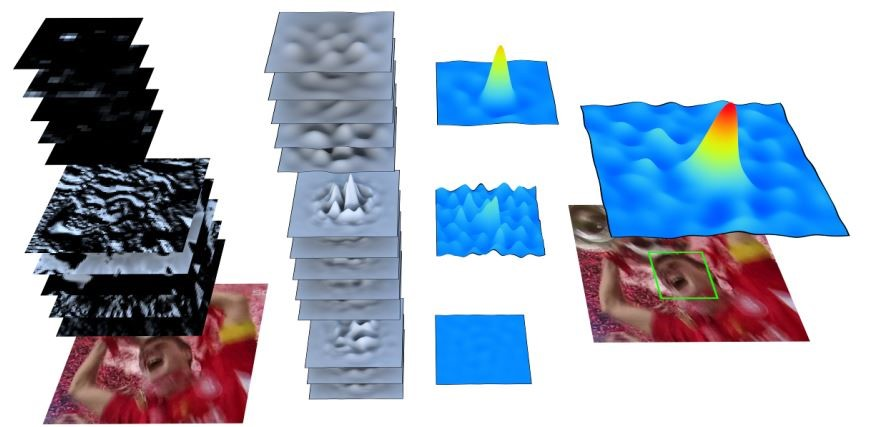
\includegraphics[width=\textwidth]{figures/RW_CCOT.jpg}
    \caption{C-COT的示意图~\cite{C-COT}}
    \label{CCOT_1}
\end{figure}

\begin{table}
    \centering
    \caption{测试用表}
    \wuhao{
    \begin{tabular}{ccc}
    \toprule[1.5pt]
        idx & +(vx,vy)+(w,h) & EAO$\uparrow$ \\ 
        \midrule[1pt]
        T-1 &  & 0.468 \\ 
        T-2 &  & 0.47 \\ 
        中文 &  & 0.471 \\ 
        T-4 &  & 0.472 \\ 
        T-5 &  & 0.479 \\ 
        T-6 & $\surd$ & 0.48 \\ 
        T-7 & $\surd$ & 0.48 \\ 
        \bottomrule[1.5pt]
    \end{tabular}
    }
    \label{CCOT_2}
\end{table}